\documentclass{sigish}
\begin{document}

% ------ Enter task number (1-3) here
\def\taskno{2}

% ------ Enter your group letter here
\def\groupno{D}

% ------ Enter your group size here
\numberofauthors{4}

% ------ Enter details for each group member here
\author{
% 1st. group member
\alignauthor J{\"u}rgen Ratzenb{\"o}ck\\
       \affaddr{Mat.nr.: 1256030}\\
       \email{juergen.ratzenboeck@gmail.com}\\ % or whichever you prefer
       \affaddr{Score Percentage: 25\%}\\ % adapt accordingly
% 2nd. group member
\alignauthor Jonathan-Edwin Asamoah\\
       \affaddr{Mat.nr.: 1457554}\\
       \email{asamoahjonathan@outlook.com}\\
       \affaddr{Score Percentage: 25\%}\\
\and
% 3rd. group member
\alignauthor Mhd Mousa Hamad\\
       \affaddr{Mat.nr.: 1556686}\\
       \email{mhd.mousa.hamad@gmail.com}\\
       \affaddr{Score Percentage: 25\%}\\
% 4th. group member
\alignauthor  Luka Vukas\\
       \affaddr{Mat.nr.: 1557457}\\
       \email{vukaslukaa@gmail.com}\\
       \affaddr{Score Percentage: 25\%}\\
}

% leave untouched!
\title{Learning from User-generated Data SS2016 -- Task \taskno}
\subtitle{Group \groupno}
\maketitle


% The following is just an example structure. Change to whatever works best for you. 
% However, make sure to include everything requested in the exercise description.

\section{Description of Task \taskno}

In this task, we should predict a set of movie ratings by adding the ratings to 200.000 (user, movie) tuples. To fulfill the task, three different datasets are provided. The first one contains 800.000 (user, movie, rating) triples which represent previous movie ratings. This file should be used in an item-based collaborative filtering approach to find the similarity between movies based on these ratings. The second file contains more information about the movies namely, title, release year and genres. This information should be used to crawl online information sources to collect more information about these movies. Then, the collected information is used to enhance the similarity results between movies, which in turns enhances the prediction accuracy. The third file contains a set of (user, movie) tuples which should finally be enriched by the predicted rating of that user for that movie.

The remainder of this paper is organized as follows. In section 2 we provide an overview and a short analysis on the provided datasets. Section 3 explains how we addressed this task and which algorithms and resources we used to compute the missing movie ratings. This section also proposes our approach to improve the results of IBCF by incorporating the information collected from external sources. Section 4 how we tested our approach using different configurations and the setups conducted for these configurations. Section 5 shows our results for different settings, and the last section wraps up the task by concluding it.

\section{Data Analysis}

The data analysis for task 2 is based on the information that was gathered in the data analysis for task 1. The results of the data analysis for task 1 involved the analysis of the training dataset, and the predict dataset. The analysis of the training dataset showed that the dataset contains 800167 (user, movie, rating) triples with the highest density at a rating of four. The analysis of the predict dataset showed that it contains 200042 (user, movie) tuples with 25 of them not part of the training dataset.
 
The new movies dataset contains 3883 (id, title, genres) triples that fit to the given data from task 1. It is used to gather additional information about the movies, three different data sources were used. Figure (\ref{fig:sources}) shows that using OMDB, we were able to gather information for 3676 movies (94\%) from the dataset, where using TMDB, 3575 movies (92\%) were enriched and finally using DBpedia, 3214 movies (82\%) were enriched by external information.

\begin{figure}
\centering
\includegraphics[width=\columnwidth]{images/sources.png}
\caption{Percentage of returned movie information}
\label{fig:sources}
\end{figure}

Based on this observation and the high density of the features, OMDB was used as the basic information source. Whereas, the other two sources were used to fill any missing information from OMDB, extend this information using other meaningful missing features and merge any available textual data to enrich it the description of the movies.

This process leads to one single dataset with 95 Features, containing the modified features form the OMDB enriched by the features from the two other sources. After removing all the features that had an extremely low density, were empty, or were highly correlated we end up with 19 features. Figure (\ref{fig:density}) shows the density for these 17 features which was used in combination with other subjective criteria to choose the final features that would be considered in our approach to predict the ratings.

\begin{figure}
\centering
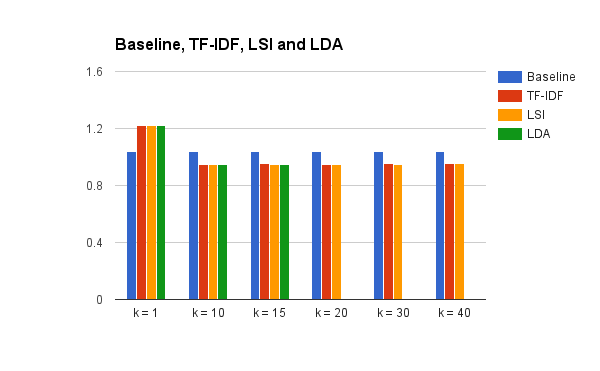
\includegraphics[width=\columnwidth]{images/density.png}
\caption{Density of Features}
\label{fig:density}
\end{figure}

\begin{figure}
\centering
\includegraphics[width=\columnwidth]{images/missing_values.png}
\caption{Percentage of missing values}
\label{fig:density}
\end{figure}

\section{Proposed Method}

For this task, we implemented a Python program that crawls three different web sources (OMDb, TMDb, Dbpedia). The program uses the crawled data along with an implemented item-based collaborative filtering algorithm to compute the missing predictions. Figure (\ref{fig:approach}) illustrates the proposed approach.

\begin{figure}
\centering
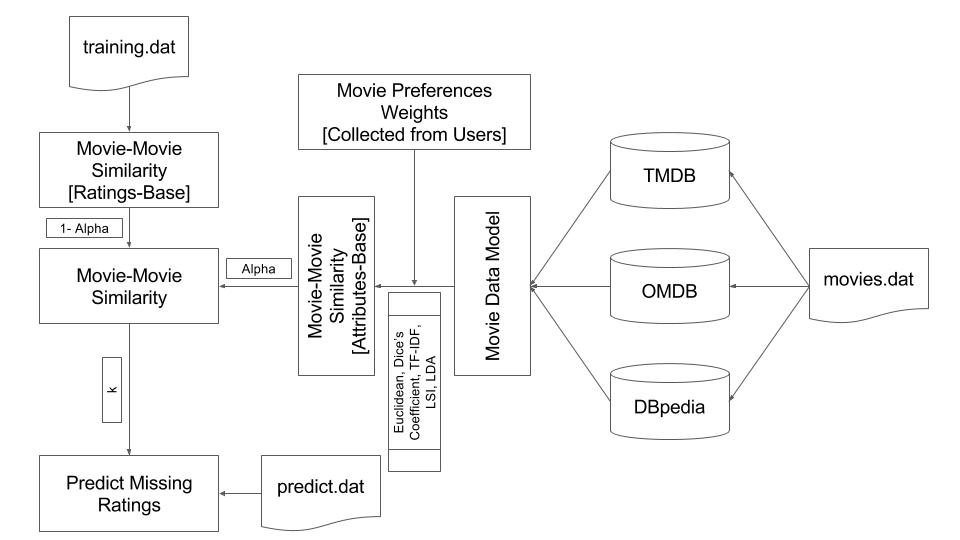
\includegraphics[width=\columnwidth]{images/system_overview.jpg}
\caption{Proposed Approach}
\label{fig:approach}
\end{figure}

\subsection{Item-Based Collaborative Filtering (IBCF)}

This approach uses the similarity between items to recommend similar items for a user or predict how would a user rate an item. When users rate an item, that item's similar items are picked from the existing system model and added to the user's recommendations. This approach is usually preferred over other memory-based approaches (user-based) when the system has more users than items as it leads to a more stable rating distribution.

Figure (\ref{fig:approach}) shows the basic steps of IBCF approach to predict how a user would rate an item. First the model has to be built by finding the similarity between all pairs of items. Then, the most similar $ k $ items which are already rated by the user are selected to compute the predicted rating of that user of the item. This computation of the rating is the average of that user's ratings for the selected items.

To find the similarity between two items, one can use previous users' ratings of these items and/or items' attributes. In this task, previous users' ratings are provided along some other attributes for movies which are the items of this task. The provided attributes for movies were enough to search for them in some public movie databases and other public resources to collect some other attributes for these movies. The similarity between two items is then calculated using a weighted sum scheme as in the following equation:
\begin{equation}
sim(x, y) = (1 - \alpha) \times sim_{r}(x, y) + (\alpha) \times sim_{a}(x, y)
\end{equation}
Where:

$ sim_{r} $ is the similarity between two movies (m1, m2) based on previous ratings

$ sim_{a} $ is the similarity between two movies (m1, m2) based on the collected attributes

$ \alpha $  is a weighting factor, in practice this factor performed best when set to (1.0), which means using only the attributes-based similarity

\subsubsection{Ratings-Based Similarity}

This similarity can take many forms, like the correlation between the compared ratings or the cosine of the angle between the vectors that are formed with these ratings. These similarity measures were explored in more details and experimented in the first task. The cosine similarity performed the best with IBCF. Therefore, it the only method that was experimented in this task.

\subsubsection{Attributes-Based Similarity}

In this task, we were provided by the title, year and genres of the movies. We used this information to crawl other information about these movies from different online open resources. The crawled information were aggregated and used to measure how movies are similar to each other.

\subsubsection*{Data Sources}

\textbf{OMDB} and \textbf{TMDB} are open movie databases accessible via custom web APIs. They provide much information about movies like for instance genres, actors, directors, writers, ratings. The provided ratings are either automatic ratings based on critics and reviews of the movies (Tomatometer from TMDB) or average user ratings collected from different sources (IMDB, TMDB).

\textbf{DBpedia} is a data-oriented interface to Wikipedia community. It combines the information spread across many Wikipedia pages into a single integrated database. This information is accessed using SPARQL which is a semantic query language for databases that store data Resource Description Framework (RDF) format. A lot of information about movies can be crawled from DBpedia using SPARQL.

\textbf{Twitter} is a popular social network which users can use to write about anything. It provides a Streaming and Search APIs to access users' posts (Tweets). The retrieved Tweets can be filtered using different keywords (Hashtags). These Tweets may contain users' reviews about movies which can be mined to extract the average ratings of movies using sentiment analysis.

OMDB, TMDB and DBpedia were crawled in this task to get more information about the movies, while Twitter was discarded as ''the Twitter Search API searches against a sampling of recent Tweets published in the past 7 days'' [According to Twitter's Search API documentation].

\subsubsection*{Similarity Measures}

The crawled information was checked and only important attributes were kept to be processed by the similarity model. These attributes were divided into seven categories:
\begin{itemize}
\item Year: contains the release year of the movie
\item Rating: contains all crawled ratings for the movie (Tomatometer, IMDB Rating, Tomato User Rating, …)
\item Genres: contains the genres of the movie
\item Stakeholders: contains all the main players in the movie production (writers, actors, directors and production companies)
\item Description: contains all text descriptions crawled from the different sources
\item Other: contains any other important features (awards, …)
\end{itemize}
For each category, a specific similarity measure is used. The similarity between two movies is calculated as a weighted sum of the similarities between their categorized attributes.

The similarity between ''Year'' and ''Rating'' attributes is measured using \textit{Euclidean Distance}. The year is a scalar value were the rating is a vector of values each of which represents different crawled rating.

The similarity between ''Genres'' and ''Stakeholders'' attributes is measured using \textit{Dice's Coefficient}. Dice's Coefficient is a common similarity method between two sets. Genres and full stakeholders' names were considered the items of the sets. This ensures that two different stakeholders with the same first or last name won't have any similarity. The similarity between stakeholders is calculated as a weighted sum of the similarities between each set of stakeholders (writers, actors, directors and production companies) using the same similarity measure.

The similarity between ''Other'' attributes is measured based on the attribute. Currently, we are considering only the awards which is measured using Dice's Coefficient.

The similarity between ''Description'' attributes is measured using one of the corpus-based similarity measures namely, Term Frequency-Inverse Document Frequency (TF-IDF), Latent Semantic Indexing (LSI) and Latent Dirichlet allocation (LDA). We defined a virtual document for each movie which is all the crawled text descriptions of it. We then used all virtual documents of all movies as our corpus to build these models.

\textbf{TF-IDF} is a numerical statistic that reflects how important a term (word) is to a document in a corpus. It is used in Vector Space Model where a matrix containing these numerical statistics for a term in a document (rows represent each document and columns represent unique terms) is constructed from a corpus. Documents are then compared by taking the cosine of the angle between the two vectors formed by any two rows.

\textbf{LSI} assumes that terms that are close in meaning will occur in similar pieces of text. A matrix containing a numerical statistic for a term in a paragraph (rows represent unique terms and columns represent each paragraph) is constructed from a corpus. Singular Value Decomposition (SVD) is used to reduce the number of rows while preserving the similarity structure among columns. Terms are then compared by taking the cosine of the angle between the two vectors formed by any two rows.

\textbf{LDA} is an example of a topic model that allows terms or documents to be represented by a set of probabilities of falling into some unobserved groups (topics). It posits that each document is a mixture of a small number of topics and that each word's creation is attributable to one of the document's topics. Terms or documents are then compared by taking the cosine of the angle between the two vectors formed by any two sets of probabilities. LDA is similar to Probabilistic LSA (pLSA).

LSA and LDA uses a predefined number of topics which represent the number of latent factors that should be extracted and used to represent the terms and documents.

\section{Experimental Setup}

As the final predictions of the task are evaluated using Root Mean Square Error (RMSE), we used this measure to evaluate our models. To make sure that the evaluation is not biased, we used 10-fold cross validation on the provided ''training.dat'' file as the true ratings are provided. Using cross-validation will ensure that no triples (user, item, rating) are used in both training (building) and evaluating the model.

Tuning all the weights automatically is not feasible as each single evaluation takes from (10-24) hours. We started by determining the weights of the attributes-based movie similarity. We setup an online excel document and asked some friends who often watch movies to order and share the preferences of selecting a movie to watch from the most important (setting its order to one) to the least important (setting its order to 9). These preferences are the attributes that we are considering in measuring the similarity between movies. Each user was given a choice to provide his name or keep it anonymous. People's preferences are kept visible to everybody. We then averaged the order of each attribute and extracted the weight of it by subtracting this average from 9. Table (\ref{tab:preferences}) shows the preferences and their average and calculated weight.

\begin{table}[]
\centering
\begin{tabular}{|l|c|c|}
\hline
\textbf{Attribute}   & \textbf{Average} & \textbf{Weight} \\ \hline
Year                 & 4.22             & 5               \\ \hline
Rating               & 3.00             & 6               \\ \hline
Genres               & 2.89             & 7               \\ \hline
Actors               & 4.00             & 5               \\ \hline
Production Companies & 6.78             & 3               \\ \hline
Directors            & 5.44             & 4               \\ \hline
Writers              & 5.44             & 4               \\ \hline
Description          & 3.11             & 6               \\ \hline
Other                & 7.89             & 2               \\ \hline  
\end{tabular}
\caption{User Preferences for Selecting Movies}
\label{tab:preferences}
\end{table}

As there is no clear documented way for selecting the number of topics (latent factors) for LSI and LDA, this parameter should be tuned automatically. Unfortunately, this was not feasible for this task due to the lack of resources. Professor Wray Buntine, Monsh University, wrote as an answer to online question\footnote{\url{https://www.quora.com/Latent-Dirichlet-Allocation-LDA-What-is-\\the-best-way-to-determine-k-number-of-topics-in-topic-modeling}} about how to set this parameter: ''With 20,000 documents using a good implementation of HDP-LDA with a Gibbs sampler I can sometimes get  K≈2000'', ''Now inspecting the 2000 topics, maybe 1600 have good quality comprehensibility''. As we have 3883 virtual documents and these virtual documents are relatively short (compared to web-page discussing a topic), we set this parameter to (150).

Fixing these parameters, we first evaluated our approach using only the attributes-based similarity between movies $ \alpha=1.0 $. The following configurations were used:
\begin{itemize}
\item \textbf{TF-IDF} with $ k = {1, 10, 15, 20, 30, 40} $
\item \textbf{LSI} with $ k = {1, 10, 15, 20, 30, 40} $
\item \textbf{LDA} with $ k = {1, 10, 15, 20, 30, 40} $
\end{itemize}

After determining the best model for corpus-based similarity (LSI) with the best $ k $ value ($ k = 15 $), we checked the results of the first task to determine which $ k $ performed the best. We compared results of each $ k $ (ratings-based and attribute-based) and fixed one value in between $ k=10 $. Fixing $ k $, we then evaluated our approach again using both similarities (ratings-based and attribute-based). The following configurations were used:
\begin{itemize}
\item $ \alpha = {0.2, 0.4, 0.6, 0.8} $
\end{itemize}

To compare the results of these different configurations, we introduced a simple mean-user-ratings approach as a baseline. This approach simply predicts the missing rating of a user for an item by averaging all his previous ratings.

\section{Results}

Table (\ref{tab:eval_00}) shows the evaluation results from the first task for IBCF using the cosine similarity measure. We can see that the best performance was at $ k = 1 $

\begin{table}[]
\centering
\begin{tabular}{|c|c|}
\hline
                & \textbf{IBCF} \\ \hline
\textbf{k = 1}  & 1.037         \\ \hline
\textbf{k = 10} & 1.115         \\ \hline
\textbf{k = 15} & 1.123         \\ \hline
\textbf{k = 20} & 1.129         \\ \hline
\textbf{k = 30} & 1.134         \\ \hline
\textbf{k = 40} & 1.135         \\ \hline
\end{tabular}
\caption{First Task Results for IBCF}
\label{tab:eval_00}
\end{table}

Table (\ref{tab:eval_01}) and Figure (\ref{fig:eval_01}) show the results of the first evaluation set along with the baseline. From them, we can see that all the tested text similarity mesures (TF-IDF, LSI, LDA) performed very closely with LSI having the best performance at $ k = 15 $.

\begin{table}[]
\centering
\begin{tabular}{|c|c|c|c|c|}
\hline
                & \textbf{Baseline} & \textbf{TF-IDF} & \textbf{LSI}   & \textbf{LDA} \\ \hline
\textbf{k = 1}  & 1.036             & 1.224           & 1.222          & 1.221            \\ \hline
\textbf{k = 10} & 1.036             & 0.948           & 0.946          & 0.947            \\ \hline
\textbf{k = 15} & 1.036             & 0.952           & \textbf{0.944} & 0.947            \\ \hline
\textbf{k = 20} & 1.036             & 0.946           & 0.947          & 0.947            \\ \hline
\textbf{k = 30} & 1.036             & 0.951           & 0.949          & 0.947            \\ \hline
\textbf{k = 40} & 1.036             & 0.954           & 0.955          & 0.947            \\ \hline
\end{tabular}
\caption{First Evaluation Set - $ \alpha = 1.0 $}
\label{tab:eval_01}
\end{table}

\begin{figure}
\centering
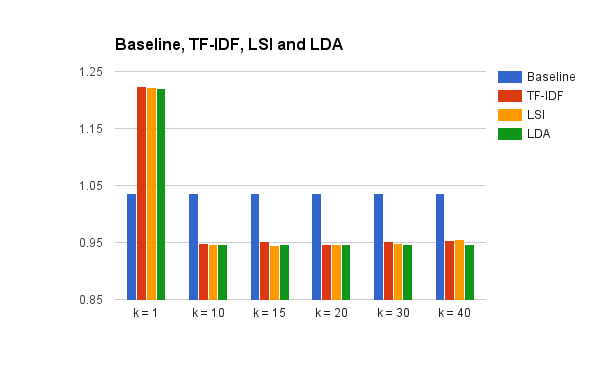
\includegraphics[width=\columnwidth]{images/evaluations.png}
\caption{First Evaluation Set - $ \alpha = 1.0 $}
\label{fig:eval_01}
\end{figure}

Table (\ref{tab:eval_02}) shows the results of the second evaluation set. In this set, we fixed $ k = 10 $ and run using only LSI model as it has the best performance in the first evaluation set. $ k = 10 $ is fixed between the best values of $ k $ in IBCF in the first and second task. It is closer to the best $ k $ in the second task as it's performance is relatively better.

\begin{table}[]
\centering
\begin{tabular}{|c|c|}
\hline
                     & \textbf{LSI} \\ \hline
\textbf{alpha = 0.0} & 1.115        \\ \hline
\textbf{alpha = 0.2} & 0.947        \\ \hline
\textbf{alpha = 0.4} & 0.948        \\ \hline
\textbf{alpha = 0.6} & 0.949        \\ \hline
\textbf{alpha = 0.8} & 0.949        \\ \hline
\textbf{alpha = 1.0} & 0.946        \\ \hline

\end{tabular}
\caption{Second Evaluation Set - $ k = 10 $}
\label{tab:eval_02}
\end{table}

\section{Conclusions}

TF-IDF, LSI and LDA were so close in their performance having LSI as the best performer in combination with $ k = 10 $. The evaluated text models didn't affect the final results much as there are other attributes affecting the similarity between two movies. Tuning all parameters for these attributes needs much more resources than we have. Although the results were close, we preferred to go with best performer to predict the final missing ratings in the file ''predict.dat''


% The following two commands are all you need in the
% initial runs of your .tex file to
% produce the bibliography for the citations in your paper.
\bibliographystyle{abbrv}
\bibliography{refs}  % refs.bib is the name of the Bibliography in this case
% You must have a proper ".bib" file
%  and remember to run:
% latex bibtex latex latex
% to resolve all references

\end{document}
